\section{Graph theory}\label{sec:graph_theory}

The term \enquote{graph} is unfortunately ambiguous\fnote{The graph of a relation or function is unrelated to the combinatorial graphs discussed here.} - it is a set of vertices connected by either directed arcs or undirected edges. \incite[362]{Knuth1997ArtVol1} states the following:
\begin{displayquote}
  Unfortunately, there will probably never be a standard terminology in this field, and so the author has followed the usual practice of contemporary books on graph theory, namely to use words that are similar but not identical to the terms used in any other books on graph theory.
\end{displayquote}

In \fullref{subsec:graphs}, we introduce distinct definitions for the four types of graphs from \cref{fig:def:graph_functors}, along with comments on how the definitions are used by different authors, and then in \fullref{def:graph_functors} we will define functors that help transparently transform some types of graphs into others. It is an established convention to not go through these hoops and implicitly transfer concepts between different kinds of graphs without even mentioning morphisms and categories. We will later follow this convention, but will nonetheless first describe the details.

The very basics overflow to \fullref{subsec:graph_walks}. After that, topics start diversifying:
\begin{itemize}
  \item \Fullref{subsec:graph_matrices} discusses graphs from the perspective of \fullref{sec:linear_algebra}.
  \item \Fullref{subsec:simple_undirected_graphs} and \fullref{subsec:graph_coloring} discuss graphs from the perspective of \fullref{sec:combinatorics}.
  \item \Fullref{subsec:trees} discuss graphs from the perspective of \fullref{sec:mathematical_logic} and \fullref{sec:computability_theory}.
  \item \Fullref{subsec:simplicial_complexes}, \fullref{subsec:quotient_graphs} and \fullref{subsec:graph_embeddings} discuss graphs from the perspective of \fullref{sec:general_topology}.
\end{itemize}

\begin{example}\label{ex:konigsberg_bridges}
  A puzzle problem regarding the seven K\"onigsberg bridges was solved by Leonhard Euler in 1735 and published six years later as \cite{Euler1741Bridges}. This is considered to be the first paper in graph theory\fnote{The early history of graph theory can be found in \cite{BiggsEtAl1986Graphs}}. In the English translation of the paper by \incite[ch. 1A]{BiggsEtAl1986Graphs}, the puzzle is described as follows in \S 2:
  \begin{displayquote}
    The problem, which I am told is widely known, is as follows: in K\"onigsberg in Prussia, there is an island \( A \). called the Kneiphof; the river which surrounds it is divided into two branches, as can be seen from \cref{fig:ex:konigsberg_bridges/schematic/drawing}, and these branches are crossed by seven bridges, \( a \), \( b \), \( c \), \( d \), \( e \), \( f \) and \( g \). Concerning these bridges, it was asked whether anyone could arrange a route in such a way that he would cross each bridge once and only once. I was told that some people asserted that this was impossible, while others were in doubt; but nobody would actually assert that it could be done. From this, I have formulated the general problem: whatever be the arrangement and division of the river into branches, and however many bridges there be, can one find out whether or not it is possible to cross each bridge exactly once?
  \end{displayquote}

  \begin{figure}[ht!]
    \frame{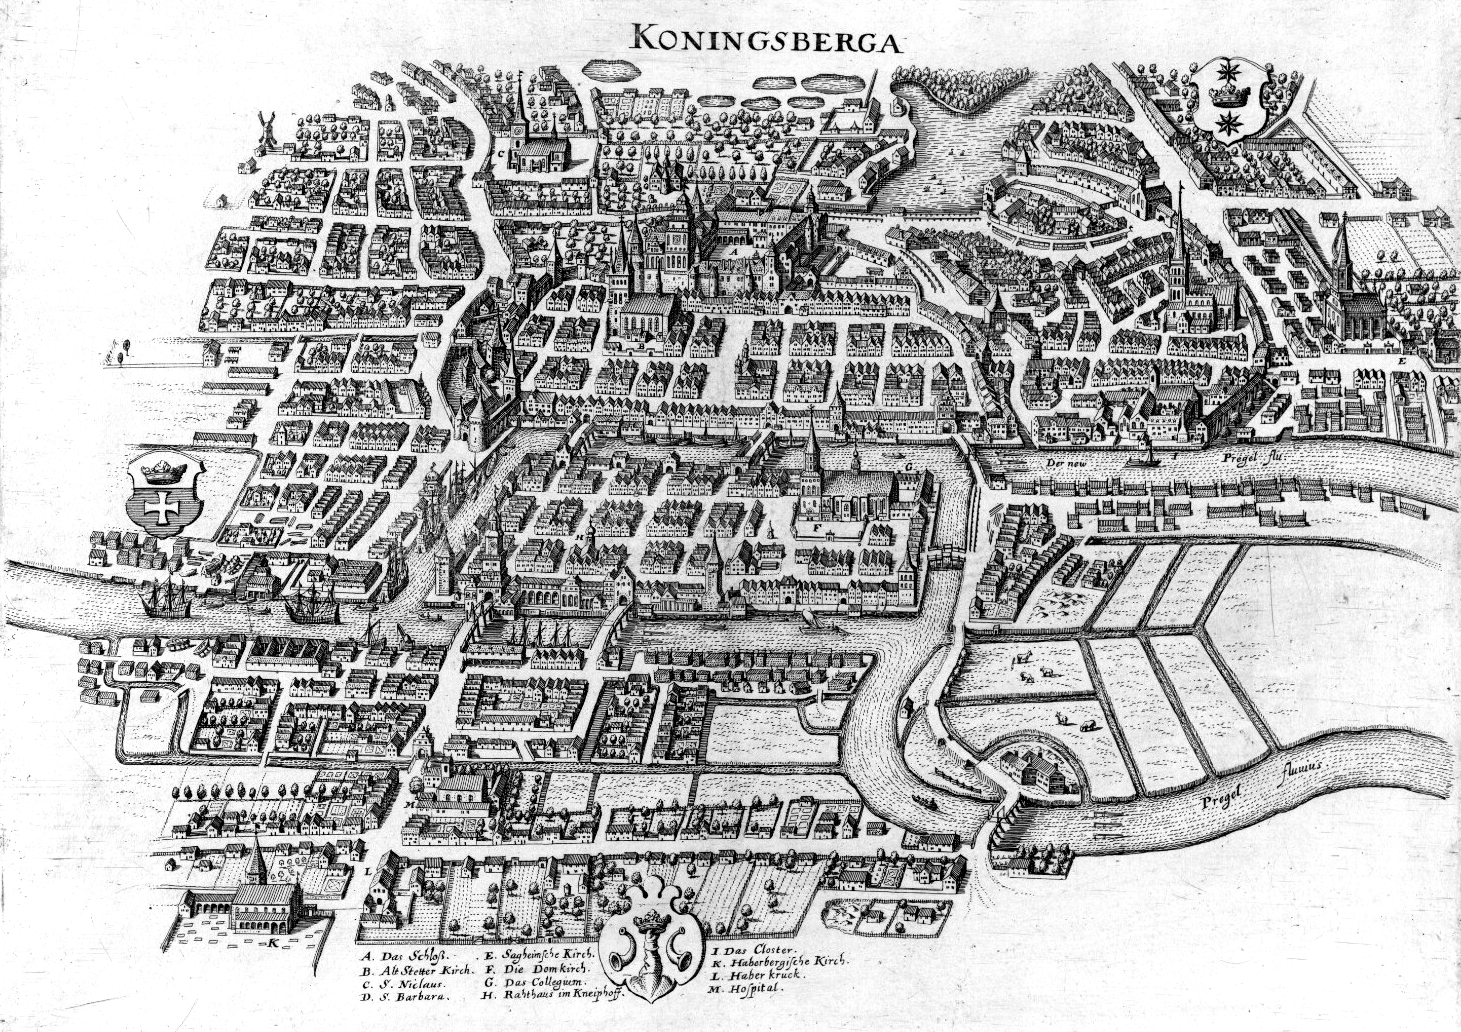
\includegraphics[width=\textwidth]{images/ex__konigsberg_bridges__illustration}}
    \caption{An illustration of K\"onigsberg by Matth\"aus Merian published in 1652 in \cite{Merian1652KönigsbergBridges}.}
    \label{fig:ex:konigsberg_bridges/illustration}
  \end{figure}

  In \S 1 of his paper, Euler himself hints at the geometric nature of the problem\fnote{Topology did not exist at the time, so the problem could not have possibly been considered topological.}:
  \begin{displayquote}
    In addition to that branch of geometry which is concerned with magnitudes, and which has always received the greatest attention, there is another branch, previously almost unknown, which Leibniz first mentioned, calling it the geometry of position. This branch is concerned only with the determination of position and its properties; it does not involve measurements, nor calculations made with them. It has not yet been satisfactorily determined what kind of problems are relevant to this geometry of position, or what methods should be used in solving them. Hence, when a problem was recently mentioned, which seemed geometrical but was so constructed that it did not require the measurement of distances, nor did calculation help at all, I had no doubt that it was concerned with the geometry of position --- especially as its solution involved only position, and no calculation was of any use. I have therefore decided to give here the method which I have found for solving this kind of problem, as an example of the geometry of position.
  \end{displayquote}

  To solve the puzzle, Euler denotes four pieces of land by \( A \), \( B \), \( C \) and \( D \) and considers sequences of adjacent pieces of land. This corresponds roughly to some modern definitions for both \enquote{walk} and \enquote{path} --- see the discussions in \fullref{rem:graph_walk_terminology}. Later, in \S 15, he even considers alternating sequences of pieces of land and bridges, which exactly corresponds to finite walks as defined in \fullref{def:graph_walk}. We will formalize the requirement of crossing each bridge exactly once by introducing Eulerian walks in \fullref{def:eulerian_walk}.

  \begin{figure}[ht!]
    \begin{subcaptionblock}{0.55\textwidth}
      \centering
      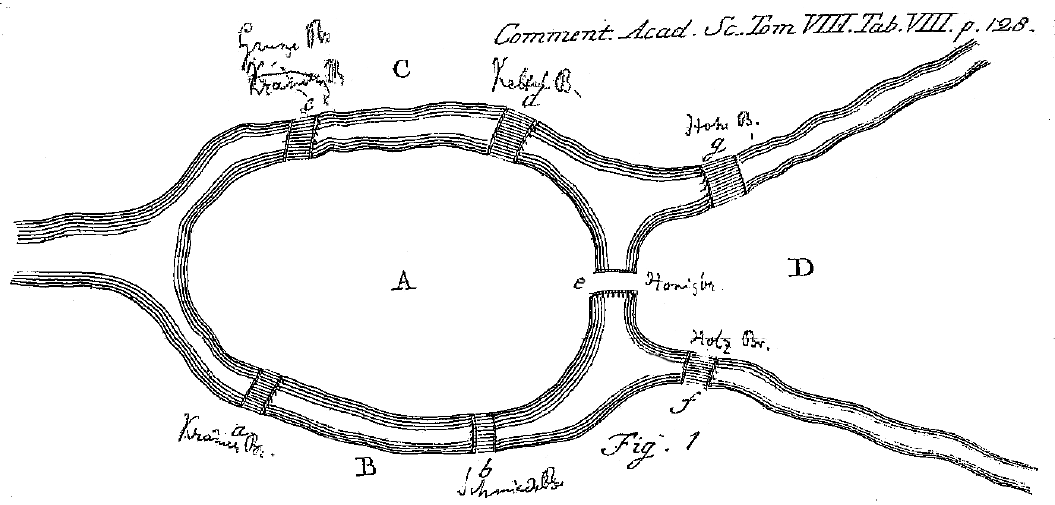
\includegraphics[width=\textwidth]{images/ex__konigsberg_bridges__schematic__drawing}
      \caption{The first figure from Euler's paper \cite{Euler1741Bridges}.}
      \label{fig:ex:konigsberg_bridges/schematic/drawing}
    \end{subcaptionblock}
    \hfill
    \begin{subcaptionblock}{0.4\textwidth}
      \centering
      \begin{equation}\label{eq:fig:ex:konigsberg_bridges/schematic/graph}
        \includegraphics[page=1]{output/ex__konigsberg_bridges}
      \end{equation}
      \caption{The corresponding \hyperref[def:hypergraph/multigraph]{undirected multigraph}.}
      \label{fig:ex:konigsberg_bridges/schematic/graph}
    \end{subcaptionblock}

    \caption{Schematic drawings of the \hyperref[ex:konigsberg_bridges]{K\"onigsberg bridges puzzle}.}\label{fig:ex:konigsberg_bridges/schematic}
  \end{figure}

  Using sequences of letters, Euler manages to reformulate the puzzle in \S 7:
  \begin{displayquote}
    The problem is therefore reduced to finding a sequence of eight letters, formed from the four letters \( A \), \( B \), \( C \) and \( D \), in which the various pairs of letters occur the required number of times. Before I turn to the problem of finding such a sequence, it would be useful to find out whether or not it is even possible to arrange the letters in this way, for if it were possible to show that there is no such arrangement, then any work directed towards finding it would be wasted. I have therefore tried to find a rule which will be useful in this case, and in others, for determining whether or not such an arrangement can exist.
  \end{displayquote}

  Euler then deduces \fullref{thm:odd_degree_vertices} in \S 16 and \S 17 and further proceeds to deduce the following rule in \S 20:
  \begin{displayquote}
    If there are more than two areas to which an odd number of bridges lead, then such a journey is impossible.

    If, however, the number of bridges is odd for exactly two areas, then the journey is possible if it starts in either of these areas.

    If, finally, there are no areas to which an odd number of bridges leads, then the required journey can be accomplished starting from any area
  \end{displayquote}

  Therefore, the K\"onigsberg bridge puzzle is resolved negatively --- no route exists that can cross each bridge in \cref{fig:ex:konigsberg_bridges/schematic/drawing} exactly once. In modern terminology, the corresponding \hyperref[def:hypergraph/multigraph]{undirected multigraph} \eqref{eq:fig:ex:konigsberg_bridges/schematic/graph} has no \hyperref[def:graph_walk/closed]{closed} \hyperref[def:eulerian_walk]{Eulerian walk} because it all of its vertices have odd \hyperref[def:graph_cardinality/undirected_degree]{degree}.

  Euler's general result is formulated with modern rigor and modern terminology and is proved in \fullref{thm:eulers_theorem_for_graphs}.
\end{example}
